\documentclass[10pt,twocolumn,letterpaper]{article}

\usepackage{statcourse}
\usepackage{times}
\usepackage{epsfig}
\usepackage{graphicx}
\usepackage{amsmath}
\usepackage{amssymb}
\usepackage{float}


% Include other packages here, before hyperref.

% If you comment hyperref and then uncomment it, you should delete
% egpaper.aux before re-running latex.  (Or just hit 'q' on the first latex
% run, let it finish, and you should be clear).
\usepackage[breaklinks=true,bookmarks=false]{hyperref}
\hypersetup{
    colorlinks=true,
    linkcolor=blue,
    filecolor=magenta,      
    urlcolor=cyan,
}


\statcoursefinalcopy


\setcounter{page}{1}
\begin{document}



%%%%%%%%%%%%%%%%%%%%%%%%%%%%%%%%%%%%%%%%%%%%%%%%%%%%%%%%%%%%%%%
% DO NOT EDIT ANYTHING ABOVE THIS LINE
% EXCEPT IF YOU LIKE TO USE ADDITIONAL PACKAGES
%%%%%%%%%%%%%%%%%%%%%%%%%%%%%%%%%%%%%%%%%%%%%%%%%%%%%%%%%%%%%%%



%%%%%%%%% TITLE
\title{\LaTeX\ Template for SBE201 Project Report}

\title{Huffman Encoding}

\author{Mostafa Mohamed Essam\\
{\tt\small mostafa.mohamed00@eng-st.cu.edu.eg}
\and
Habiba Mahmoud Abdelhalim\\
{\tt\small habiba.ahmed98@eng-st.cu.edu.eg}
\and
Mo'men Maged Mohamed\\
{\tt\small momen.rizk99@eng-st.cu.edu.eg}
\and
Mariam Mohamed Osama\\
{\tt\small mariam.hamed99@eng-st.cu.edu.eg}
\and
Anas Mohamed Abdelrahman\\
{\tt\small fakestar.anas19019@gmail.com}

}

\maketitle
%\thispagestyle{empty}



% MAIN ARTICLE GOES BELOW
%%%%%%%%%%%%%%%%%%%%%%%%%%%%%%%%%%%%%%%%%%%%%%%%%%%%%%%%%%%%%%%



%%%%%%%%% BODY TEXT




\section{Introduction}

In 1951, the MIT student David A. Huffman was working on his term paper which his professor gave to Huffman's class for whom didn't want to take the final exam.
The Problem that was assigned to them was to find the most effecient binary code. Huffman got the idea to use a frequency sorted binary tree and proved that his method is the most efficient.\cite{1991SciAm.265c..54S}
\\
Huffman coding assigns binary codes to character in such a way that the code's lenght depends on the frequency/weight of its corresponding character.
The codes have variable lenghths, and they're prefix-free which means that any code isn't a prefix of any of the other codes.\cite{huffman_encoding_2014} 
\\
The Huffman tree is a binary tree in which any leaf in the tree corresponds to the character/data that is being coded.
\\
We have managed to utilize this technique to compress images with ".pgm" format by encoding each pixel in the image according to its frequency thus storing it in less number of bits.

\begin{figure}[H]
\begin{center}
   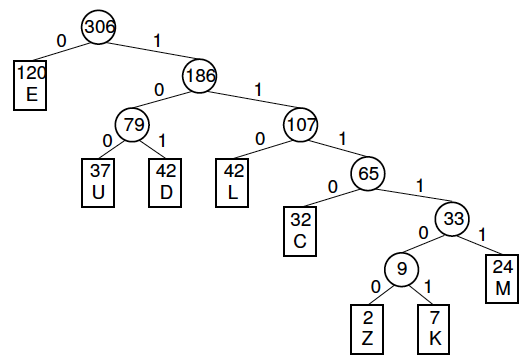
\includegraphics[width=0.8\linewidth]{Huffman-tree-Fig5.24.png}
\end{center}
   \caption{Example of a coded Huffman Tree}
\label{fig: Huffman Tree}
\end{figure}

\section{Motivation}
We were really motivated and enthusiastic about this project cause it helped us learn a lot of new things:
\begin{enumerate}
   \item The concept of file compression and how much useful it is.
   \item How to read/write files using \verb!C++!.
   \item How to handle command line arguments and flags.
   \item Storing data in binary files.
   \item Learned how useful some data structures like hashmaps are.
   \item How to make user friendly GUI with a descent UI.
\end{enumerate}


\section{Resources}
We used the \href{https://people.sc.fsu.edu/~jburkardt/c_src/pgmb_io/pgmb_io.html}{pgmb\textunderscore io} library to read and write the pgm file.
Its written mainly in c, we added more c++ functionalities to make it compatible with our application and we removed the unneeded functions in it.

\section{Challenges and Problems}
\begin{enumerate}
   \item Learning how to use fstream functionalities.
   \item Learning how to build a GUI.
   \item Converting data to bitsets.
\end{enumerate}
\section{System Block Diagram}
\begin{figure}[H]
   \begin{center}
      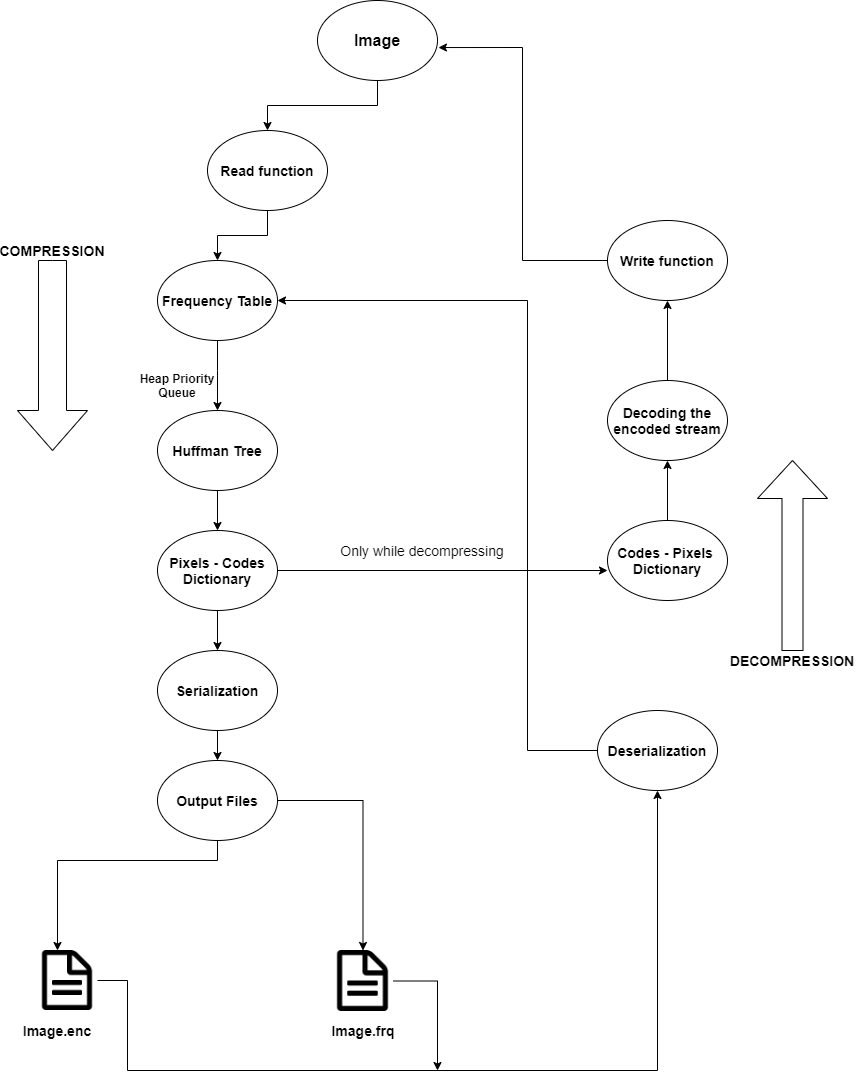
\includegraphics[width=1\linewidth]{Block_Diagram.png}
   \end{center}
      \caption{System Block Diagram}
   \label{fig: Block Diagram}
   \end{figure}

\section{User manual for the system}

Steps to run your programs.


\section{Results}

Screenshots for your running programs

\section{Contributions}
\begin{enumerate}
   \item Mostafa Essam: \begin{enumerate}
      \item Read/write imagefiles in ".pgm" format. 
      \item Serializing the encoded image and frequency table.
      \item Deserializing the frequency table.
      \item Documentation
   \end{enumerate}
   \item Habiba Mahmoud: \begin{enumerate}
      \item Construct a frequency table from the image. 
      \item From the frequency table,construct Huffman tree with the help of heap priority queue (Huffman Encoding).
      \item Generate the codes for each pixel.
      \item Documentation.
   \end{enumerate}
   \item Mo'men Maged: \begin{enumerate}
      \item Deserializing the encoded image and frequency table.
      \item Decoding the encoded image data.
      \item Arguments flag.
      \item Report.
   \end{enumerate}
   \item Mariam Mohamed Osama: GUI.
   \item Anas Mohamed Abdelrahman: GUI.
\end{enumerate}

{\small

\bibliographystyle{IEEEtran}
\bibliography{bibliography.bib}
}

\end{document}